\documentclass[a4paper,
fontsize=11pt,
%headings=small,
oneside,
numbers=noperiodatend,
parskip=half-,
bibliography=totoc,
final
]{scrartcl}

\usepackage{synttree}
\usepackage{graphicx}
\setkeys{Gin}{width=.4\textwidth} %default pics size

\graphicspath{{./plots/}}
\usepackage[ngerman]{babel}
\usepackage[T1]{fontenc}
%\usepackage{amsmath}
\usepackage[utf8x]{inputenc}
\usepackage [hyphens]{url}
\usepackage{booktabs} 
\usepackage[left=2.4cm,right=2.4cm,top=2.3cm,bottom=2cm,includeheadfoot]{geometry}
\usepackage{eurosym}
\usepackage{multirow}
\usepackage[ngerman]{varioref}
\setcapindent{1em}
\renewcommand{\labelitemi}{--}
\usepackage{paralist}
\usepackage{pdfpages}
\usepackage{lscape}
\usepackage{float}
\usepackage{acronym}
\usepackage{eurosym}
\usepackage[babel]{csquotes}
\usepackage{longtable,lscape}
\usepackage{mathpazo}
\usepackage[normalem]{ulem} %emphasize weiterhin kursiv
\usepackage[flushmargin,ragged]{footmisc} % left align footnote
\usepackage{ccicons} 

%%%% fancy LIBREAS URL color 
\usepackage{xcolor}
\definecolor{libreas}{RGB}{112,0,0}

\usepackage{listings}

\urlstyle{same}  % don't use monospace font for urls

\usepackage[fleqn]{amsmath}

%adjust fontsize for part

\usepackage{sectsty}
\partfont{\large}

%Das BibTeX-Zeichen mit \BibTeX setzen:
\def\symbol#1{\char #1\relax}
\def\bsl{{\tt\symbol{'134}}}
\def\BibTeX{{\rm B\kern-.05em{\sc i\kern-.025em b}\kern-.08em
    T\kern-.1667em\lower.7ex\hbox{E}\kern-.125emX}}

\usepackage{fancyhdr}
\fancyhf{}
\pagestyle{fancyplain}
\fancyhead[R]{\thepage}

% make sure bookmarks are created eventough sections are not numbered!
% uncommend if sections are numbered (bookmarks created by default)
\makeatletter
\renewcommand\@seccntformat[1]{}
\makeatother


\usepackage{hyperxmp}
\usepackage[colorlinks, linkcolor=black,citecolor=black, urlcolor=libreas,
breaklinks= true,bookmarks=true,bookmarksopen=true]{hyperref}
%URLs hart brechen
\makeatletter 
\g@addto@macro\UrlBreaks{ 
  \do\a\do\b\do\c\do\d\do\e\do\f\do\g\do\h\do\i\do\j 
  \do\k\do\l\do\m\do\n\do\o\do\p\do\q\do\r\do\s\do\t 
  \do\u\do\v\do\w\do\x\do\y\do\z\do\&\do\1\do\2\do\3 
  \do\4\do\5\do\6\do\7\do\8\do\9\do\0} 
% \def\do@url@hyp{\do\-} 
\makeatother 

%meta
%meta

\fancyhead[L]{V. Burtscher et al. \\ %author
LIBREAS. Library Ideas, 33 (2018). % journal, issue, volume.
\href{http://nbn-resolving.de/}
{}} % urn 
% recommended use
%\href{http://nbn-resolving.de/}{\color{black}{urn:nbn:de...}}
\fancyhead[R]{\thepage} %page number
\fancyfoot[L] {\ccLogo \ccAttribution\ \href{https://creativecommons.org/licenses/by/3.0/}{\color{black}Creative Commons BY 3.0}}  %licence
\fancyfoot[R] {ISSN: 1860-7950}

\title{\LARGE{Jugendteam -- Partizipationsmöglichkeit Jugendlicher in öffentlichen Bibliotheken}} % title
\author{Verena Burtscher, Bibliotheksmitarbeiterinnen im Jugendteam \\ der Walserbibliothek Raggal (Franziska, Julia, Helena, Viktoria, \\ Janine, Nina, Luisa, Leonie, Leonora, Mia)} % author

\setcounter{page}{1}

\hypersetup{%
      pdftitle={Jugendteam -- Partizipationsmöglichkeit Jugendlicher in öffentlichen Bibliotheken},
      pdfauthor={Verena Burtscher, Bibliotheksmitarbeiterinnen im Jugendteam der Walserbibliothek Raggal (Franziska, Julia, Helena, Viktoria, Janine, Nina, Luisa, Leonie, Leonora, Mia)},
      pdfcopyright={CC BY 3.0 Unported},
      pdfsubject={LIBREAS. Library Ideas, 33 (2018).},
      pdfkeywords={Bibliothek, Berufspraxis, Jugend, Beteiligung, Österreich},
      pdflicenseurl={https://creativecommons.org/licenses/by/3.0/},
      pdfcontacturl={http://libreas.eu},
      baseurl={http://libreas.eu},
      pdflang={de},
      pdfmetalang={de}
     }



\date{}
\begin{document}

\maketitle
\thispagestyle{fancyplain} 

%abstracts

%body
\hypertarget{das-jugendteam-der-walserbibliothek-raggal}{%
\section*{Das Jugendteam der Walserbibliothek
Raggal}\label{das-jugendteam-der-walserbibliothek-raggal}}

\emph{Franziska, Julia, Helena, Viktoria, Janine, Nina, Luisa, Leonie,
Leonora, Mia}

Wir sind derzeit zehn Kinder und Jugendliche zwischen 8 und 17 Jahren
und bilden das Jugendteam der öffentlichen Bibliothek
\enquote{Walserbibliothek Raggal} (Vorarlberg/Österreich). Die
Hauptaufgabe unseres Teams besteht in der eigenverantwortlichen
Organisation, Koordination und Gestaltung der speziell eingeführten
Jugendöffnungszeiten jeden Freitag von 17.00 bis 18.30 Uhr. Zudem
gestalten wir selbst kleine Veranstaltungen für Jugendliche, werden an
der Entscheidungsfindung, der Planung und Durchführung von
Veranstaltungen für Kinder und Jugendliche aktiv beteiligt und führen
von Zeit zu Zeit Projekte durch (aktuelles Projekt:
\enquote{Plastiktaschen RAUS -- Stofftaschen REIN}\footnote{\url{http://www.walserbibliothek.at/plastiktaschen-raus-stofftaschen-rein}}).
Wir unterstützen das Bibliotheksteam bei seiner Arbeit und helfen aus,
wenn es Engpässe bei der Abdeckung der Öffnungszeiten oder durch
Ausfälle von Mitarbeiterinnen gibt. Betreut werden wir von der
Bibliotheksleiterin, die vor allem die Koordination und
Informationsweitergabe zwischen dem Jugend- und dem Bibliotheksteam
(Teamsitzung) übernimmt. Zur Eigenständigkeit des Jugendteams gehört
auch ein eigenes Budget für Medieneinkäufe und Veranstaltungen und
vollkommene Entscheidungsfreiheit.

Die Anforderungen, die an uns junge Bibliothekarinnen gestellt werden,
sind Selbständigkeit in der Durchführung der gesamten Bibliotheksarbeit
sowie spontane und kreative Eigeninitiative in der Gestaltung der
Jugendöffnungszeiten und bei Veranstaltungen für Jugendliche.

Wir arbeiten gerne im Jugendteam der Walserbibliothek, weil uns die
Bibliotheksarbeit Spaß macht, weil wir mitbestimmen und gestalten
dürfen, weil wir viel gemeinsam erleben, weil es da so viele spannende
Medien gibt, weil die Bibliothek ein Treffpunkt ist...

\begin{figure}
\centering
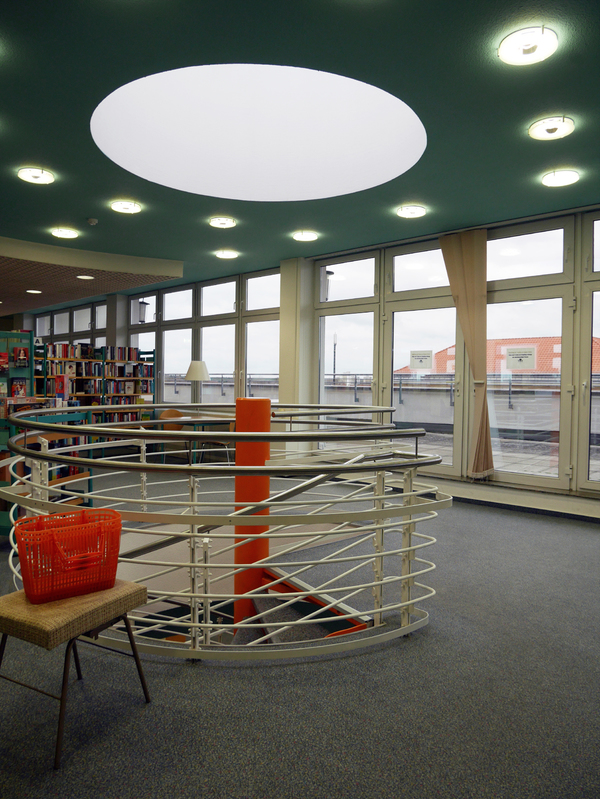
\includegraphics{image_1.jpg}
\caption{Das Jugendteam: Franziska, Julia, Helena, Viktoria, Janine,
Nina, Luisa, Leonie, Leonora, Mia}
\end{figure}

\newpage

\hypertarget{die-sicht-der-bibliothek}{%
\section*{Die Sicht der
Bibliothek}\label{die-sicht-der-bibliothek}}

\emph{Verena Burtscher}

Klaudia Büchel ist seit 2002 als ehrenamtliche Bibliotheksleiterin in
der Walserbibliothek Raggal tätig und gründete im Jahre 2004 ein
\emph{Jugendteam}, welches seither fester Bestandteil der Bibliothek
ist. Sie ist überzeugt, dass eine derart gestaltete Partizipation die
Integration einer \enquote{Jugendbibliothek} vor allem in kleineren
Bibliotheken mit begrenzten Räumlichkeiten ermöglicht. So wird die
Bibliothek zum Freizeitort für Jugendliche und es kann auf deren
besonderen Bedürfnisse und aktuellen Anforderungen gezielt eingegangen
werden.

Die Jugendbibliotheksarbeit dient als Freizeitgestaltung und wirkt sich
insofern positiv aus, dass das Medienangebot verstärkt in Anspruch
genommen wird und die Jugendteammitglieder ihre Familien und Freunde mit
Medien versorgen. Der selbstbestimmte Ankauf von Medien durch die
Jugendlichen, unter Berücksichtigung der Buchwünsche Jugendlicher,
animiert verstärkt auch andere Jugendliche zum Lesen. Zudem fördert die
gemeinsame Bibliotheksarbeit die Medien- und Sozialkompetenz und
ermöglicht das Kennenlernen und Mitgestalten von Organisationsprozessen.
\textbf{Die Bibliotheksarbeit durch Jugendliche macht die Bibliothek zum
Freizeitort und wirkt sich positiv auf das Nutzungsverhalten, die
Nutzungsfrequenz und die Lesemotivation Jugendlicher aus.}

\begin{figure}
\centering
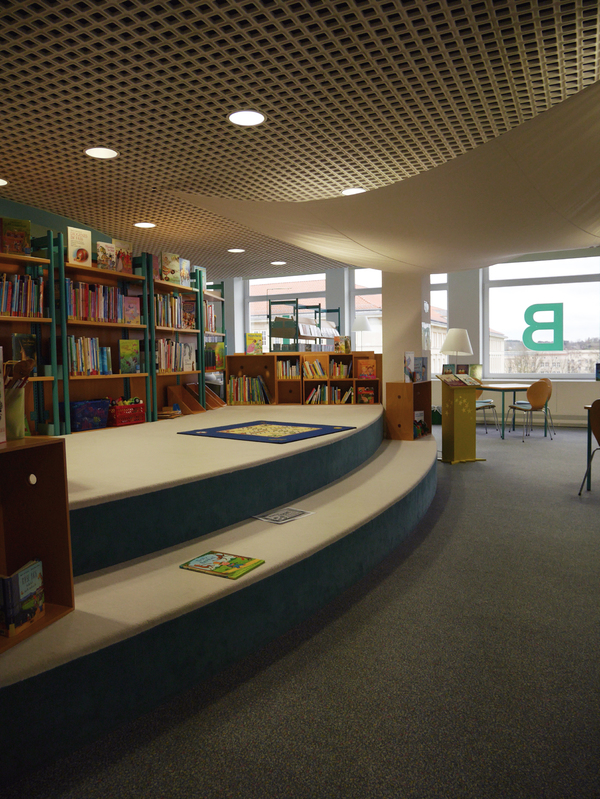
\includegraphics{image_2.jpg}
\caption{Monatliche Teamsitzung des Jugendteams}
\end{figure}

Die ehrenamtliche Bibliotheksarbeit im Jugendteam stärkt zudem das
Selbstvertrauen der Jugendlichen im Umgang mit verschiedensten Medien,
in der Ausführung der selbständigen Bibliotheksarbeit sowie im Auftreten
gegenüber anderen. Das Zugehörigkeitsgefühl hat vor allem bei jüngeren
Teammitgliedern und da besonders bei Kindern aus eher bildungsfernen
Familien eine besondere Bedeutung. Die gemeinschaftliche
Bibliotheksarbeit erfordert Teamfähigkeit sowie Verlässlichkeit und
fördert die Sozial-, Medien- und Informationskompetenz der Jugendlichen.
Die Eigeninitiative zu sozialem Engagement wird gefördert und hält auch
über das Jugendteam hinaus an, was sich in der Vorbildfunktion und
Verantwortungsübernahme ehemaliger Mitglieder für das Jugendteam zeigt,
die von sich aus neue Mitglieder schulen und beratend zur Seite stehen.
Die Bibliothek als Freizeitort sowie die Betreuung in den
Jugendöffnungszeiten durch das Jugendteam fördert die Kommunikation
unter Jugendlichen und hat Auswirkungen auf die Sozialkompetenz anderer
Jugendlicher, die freiwillig in der Bibliothek oder bei Veranstaltungen
mithelfen und sich bei Projekten sozial engagieren. \textbf{Die
ehrenamtliche Arbeit in der Bibliothek fördert die Sozial-, Medien- und
Informationskompetenz sowie die Kommunikation unter Jugendlichen und
wirkt sich positiv auf das soziale Engagement aus.}

Aus Sicht der Bibliotheksleiterin ergeben sich durch ein integriertes
Jugendteam für die Bibliothek vielfältige Möglichkeiten und Chancen.
Jugendliche wecken Interesse an der Bibliothek und an der
Bibliotheksarbeit und sind Informationsträger in der Öffentlichkeit.
Frühe und positive Bibliothekserfahrungen entwickeln ein Bewusstsein für
die Bibliothek, welches bis ins Jugendalter und darüber hinaus anhält
und fördern so die langfristige Bindung als Nutzer. Jugendliche wissen
am besten, wie sich Jugendliche ihre Bibliothek vorstellen und was sie
sich wünschen, weshalb die Bibliothek passende Nutzungsmöglichkeiten und
interessante Angebote für Jugendliche anbieten kann. Die
Bibliotheksarbeit durch Jugendliche hinterlässt ein positives
Bibliotheksimage bei Familien und Jugendlichen. Jugendliche als
Potential für die Bibliotheksarbeit zu erkennen, bedeutet nicht nur
Entlastung und Unterstützung des Bibliotheksteams, sondern auch, dass
vor allem die ehrenamtliche Bibliotheksarbeit durch ausreichenden
Nachwuchs gesichert werden kann. Wichtig dabei ist die Abgabe von
Verantwortung an Jugendliche. Die selbständige Bibliotheksarbeit eines
Jugendteams ist eine Möglichkeit, Lesen und Bibliothek als
Selbstverständlichkeit im Leben von Kindern und Jugendlichen zu
integrieren und so Einfluss auf die Lesemotivation durch positive
Bibliothekserfahrungen zu nehmen. Ein Jugendteam soll die Bibliothek als
Treffpunkt, als Lernort, als Gestaltungs- und Erfahrungsraum für
Jugendliche weiter etablieren. Ein leichter, unkomplizierter
Medienzugang für alle und die Betreuung durch das Jugendteam als
Vorbilder für Kinder und Jugendliche sollen das Lesen fördern und Bücher
und Literaturvermittlungsangebote speziell für die Zielgruppe
Jugendliche attraktiver machen.

Weitere Informationen auf:

\url{http://www.raggal.bvoe.at/jugendbibliothek}

\url{http://www.raggal.bvoe.at/leitpapier-jugendteam}

%autor
\begin{center}\rule{0.5\linewidth}{\linethickness}\end{center}

\textbf{Verena Burtscher}, Bibliothekarin in der Walserbibliothek
Raggal.

\end{document}
